\subsection{Evaluaci\'on de desempe\~no del software en pruebas iniciales 1}
    El apartado de desempe\~no del software es complicado de
        medir, debido a que el \'unico caso en el que se puede
        observar si hay una mejora o no es con el tiempo en el cual
        se realiza la simulaci\'on.
    \vskip 0.5cm
    Este tiempo puede variar en cada una de las ejecuciones del
        programa sin importar si las condiciones iniciales son las
        mismas, debido a que existe un grado de aleatoriedad
        inherente al algoritmo, por lo que cada una de las rutas que
        pueden llegar a ser obtenidas por el simulador var\'ian en cada
        una de las ejecuciones, como se puede comprobar al observar
        las Figuras \ref{fig:Ruta 1} - \ref{fig:Ruta 5}.
    \vskip 0.5cm
    %figura
    \begin{figure}[htbp]
        \centering
        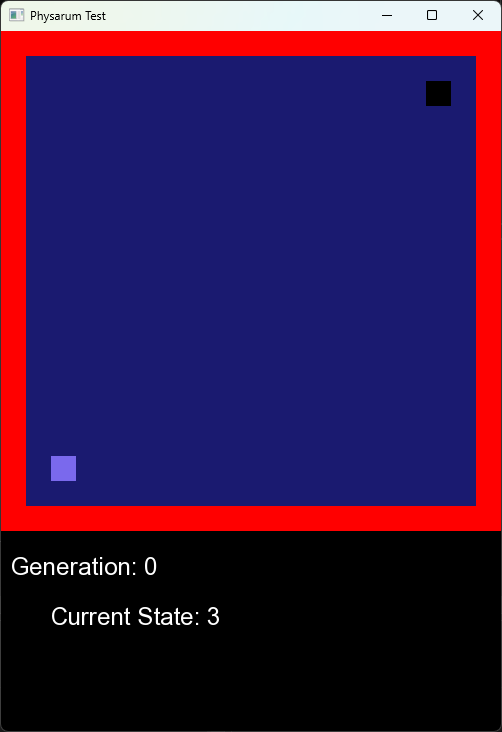
\includegraphics[width=0.5\textwidth]{./images/Pruebas/simulador/image009.png}
        \caption{Configuraci\'on Base}
        \label{fig:Ruta 1}
    \end{figure}
    \vskip 0.5cm
    %figura
    \begin{figure}[htbp]
        \centering
        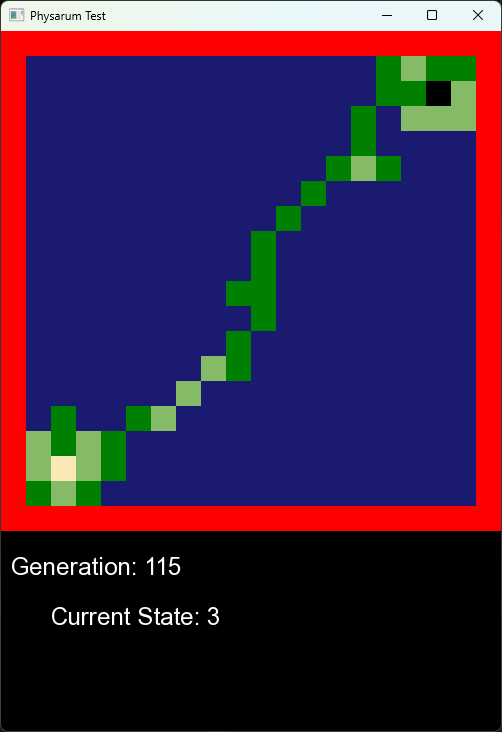
\includegraphics[width=0.5\textwidth]{./images/Pruebas/simulador/image011.png}
        \caption{Primera Ruta Obtenida}
        \label{fig:Ruta 2}
    \end{figure}
    \vskip 0.5cm
    %figura
    \begin{figure}[htbp]
        \centering
        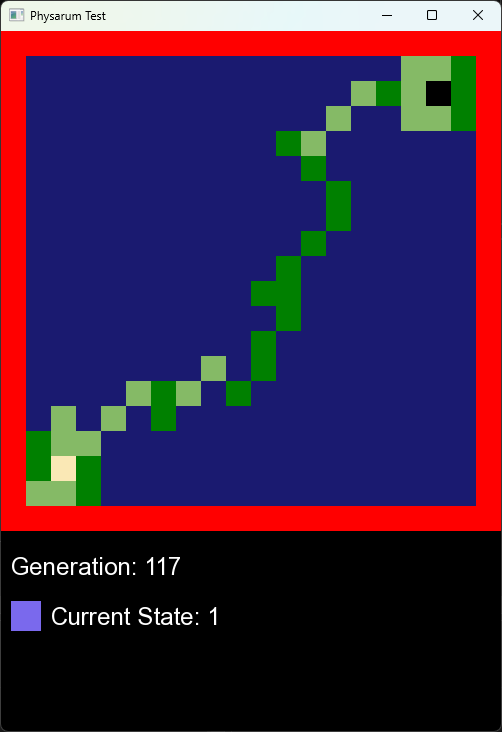
\includegraphics[width=0.5\textwidth]{./images/Pruebas/simulador/image013.png}
        \caption{Segunda Ruta Obtenida}
        \label{fig:Ruta 3}
    \end{figure}
    \vskip 0.5cm
    %figura
    \begin{figure}[htbp]
        \centering
        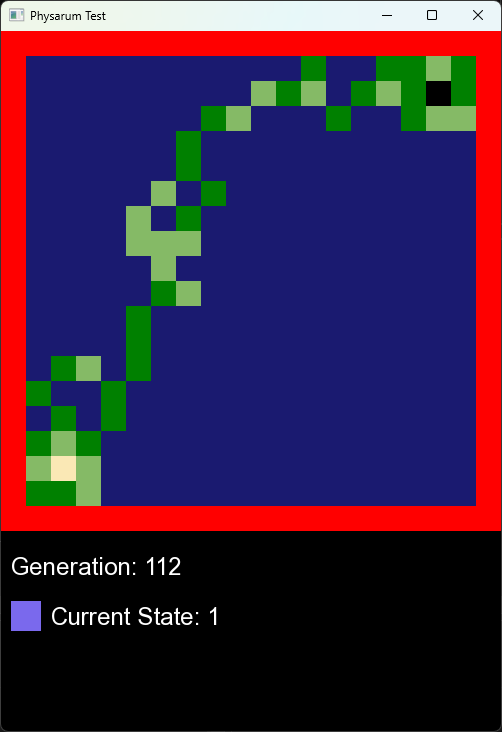
\includegraphics[width=0.5\textwidth]{./images/Pruebas/simulador/image015.png}
        \caption{Tercera Ruta Obtenida}
        \label{fig:Ruta 4}
    \end{figure}
    \vskip 0.5cm
    %figura
    \begin{figure}[htbp]
        \centering
        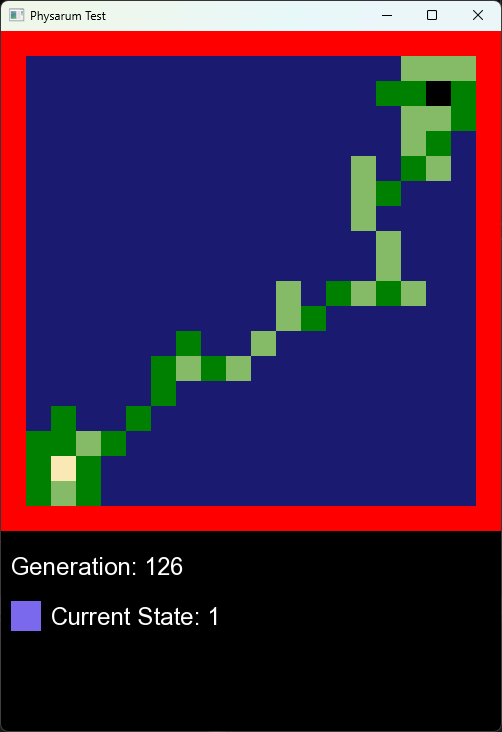
\includegraphics[width=0.5\textwidth]{./images/Pruebas/simulador/image017.png}
        \caption{Cuarta Ruta Obtenida}
        \label{fig:Ruta 5}
    \end{figure}
    \vskip 0.5cm
    \clearpage
    Como se puede comprobar, a pesar de que el estado inicial
        sea exactamente el mismo, la ruta obtenida a partir del
        simulador cambia en cada uno de los casos, por lo que medir
        el tiempo en el que se es obtenida la ruta se vuelve inviable,
        ya que cada una de las rutas que puede ser generada puede
        llegar a tardar mayor o menor tiempo de acuerdo a las
        generaciones que sean necesarias para terminar por
        obtenerla.
    \vskip 0.5cm
    Debido a lo anterior, se consider\'o otra forma de medir el
    tiempo de ejecuci\'on del programa para analizar su
    desempe\~no, es evaluar el tiempo de ejecuci\'on entre una
    generaci\'on y la siguiente. Al ser evaluada una matriz de
    tama\~no n x n, donde en cada una se eval\'uan una serie de
    condiciones para determinar el valor que contiene dicha
    celda, hay una diferencia de tiempo entre cada evaluaci\'on de
    la matriz mientras pasa cada una de las generaciones, por lo
    que se vuelve conveniente usar esta diferencia de tiempo
    como un par\'ametro de evaluaci\'on del desempe\~no para el
    algoritmo.
    \vskip 0.5cm
    Durante las pruebas de funcionamiento iniciales del
        programa, tambi\'en se encontr\'o que existe una diferencia de
        desempe\~no en su ejecuci\'on entre Windows y Linux, por lo
        que para la recopilaci\'on de informaci\'on y datos recabados se
        debe de tomar en cuenta las ejecuciones en ambos sistemas
        operativos, debido a que pueden existir diferencias
        significativas a pesar de que las condiciones iniciales sean
        similares entre s\'i.
% subsection Evaluaci\'on de desempe\~no del software en pruebas iniciales (end)